\section{Introduction and Motivation}

	\begin{frame}
		\frametitle{Introduction}
		\begin{columns}
			\begin{column}{0.49\textwidth}
				\begin{itemize}
					\item \onslide<1->{Novel Strategy} \\[0.7cm]
					\item \onslide<2->{Decentralized Navigation} \\[0.7cm]
					\item \onslide<3->{Optimal Motion Planning} \\[0.7cm]
					\item \onslide<5->{Autonomous Decision Making}
				\end{itemize}
			\end{column}
			\pause
			\begin{column}{0.49\textwidth}
				\centering
				\onslide<4->{\includegraphics[width=0.85\textwidth]{pictures/robot_comic.png}}
			\end{column}
		\end{columns}
	\end{frame}
	
	\begin{frame}
		\frametitle{Latest Approaches and Motivation}
	    \begin{columns}[T]
	        \begin{column}{0.49\textwidth}
	            \begin{itemize}%[<+->] Kommentar entfernen falls jeder Punkt einzeln erscheinen soll
					\item \onslide<1->{Environment Previous Knowledge}\\[0.5cm]
					\item \onslide<3->{Maximum speed $\leq 1.5 m/s$} \\[1cm]
					\item \onslide<4->{This approach has the potential to improve : \\[0.5cm]
					\begin{itemize}
						\item system performance \\[0.2cm]
						\item fast path towards goal
					\end{itemize}
					}
	        	\end{itemize}
	        \end{column}
	        \begin{column}{0.49\textwidth}
	        	\begin{itemize}%[<+->] Kommentar entfernen falls jeder Punkt einzeln erscheinen soll
	        		\item \onslide<2->{Global Planner}
	        	\end{itemize}
        		\centering
        		\only<1>{\includegraphics[width=0.8\textwidth]{pictures/figure_1.png}}
        		\only<2>{\includegraphics[width=0.8\textwidth]{pictures/figure_2.png}}
        		\only<3->{\includegraphics[width=0.8\textwidth]{pictures/figure.png}}
	        \end{column}
	    \end{columns}
	\end{frame}
	
	\begin{frame}
		\begin{block}{Proposed Approach\footnotemark}
			\begin{itemize}
				\pause
				\item On-line trajectory planning \\ [0.4cm]
				\pause
				\item Without \textit{global planner} \\ [0.4cm]
				\pause
				\item Without \textit{map} \\ [0.4cm]
				\pause
				\item Dynamic Environment, e.g. \textit{(pedestrian, multi-robots)} \\ [0.4cm]
				\pause
				\item Robot speed $> 1.5 m/s$ \\ [0.4cm]
				\pause
				\item Smooth navigation \\ [0.4cm]
				\pause
				\item Deadlock free
			\end{itemize}
		\end{block}
		\footnotetext[1]{
			Hoy, Michael and Matveev, Alexey S. and Savkin, Andrey V. 
			\say{
				\href{https://www.cambridge.org/core/journals/robotica/article/algorithms-for-collisionfree-navigation-of-mobile-robots-in-complex-cluttered-environments-a-survey/ADA8F6F7E30123629A26B08DA0C79C8C}{
					\textcolor{tudark}{Algorithms for collision-free navigation of mobile robots in complex cluttered environments: a survey}
				}
			}. In Cambridge University Press (2016).
		}
	\end{frame}

	\begin{frame}
		\begin{columns}[T]
			\begin{column}{0.49\textwidth}
			\begin{itemize}%[<+->] Kommentar entfernen falls jeder Punkt einzeln erscheinen soll
				\item Current Approach: \\[0.2cm]
				\begin{itemize}
					\item Laser Scanner + Map \\[0.1cm]
					\item Robot's estimated location 
				\end{itemize}
			\end{itemize}
			\includegraphics[scale=0.67]{pictures/navigation_ros_2.pdf}
			\end{column}
			\pause
			\begin{column}{0.49\textwidth}
				\begin{itemize}%[<+->] Kommentar entfernen falls jeder Punkt einzeln erscheinen soll
					\item Proposed Approach: \\[0.2cm]
					\begin{itemize}
						\item Robot localization \\[0.1cm]
						\item Obstacles location 
					\end{itemize}
				\end{itemize}
				\includegraphics[scale=0.75]{pictures/navigation_ros_3.pdf}
			\end{column}
		\end{columns}
	\end{frame}

	\begin{frame}
		\frametitle{Model Predictive Control}
		\centering
		\only<1>{\animategraphics[loop,controls,width=0.75\textwidth]{2}{pictures/mpc_group/MPC_scheme_basic-}{0}{6}}
		\only<2>{\includegraphics[scale=1.0]{pictures/mpc_group/MPC_scheme_basic-7.pdf}}
	\end{frame}

	\begin{frame}
		\frametitle{On-line Trajectory (prediction horizon)}
		\centering
		\movie[width=0.42\textwidth, height=0.45\textwidth]
		{\includegraphics[width=0.42\textwidth]{pictures/path.png}}{videos/path.mov}
	\end{frame}

	\begin{frame}
		\frametitle{NMPC Optimization Problem Schematic}
		\centering
		\only<1>{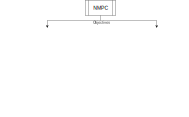
\includegraphics[scale=0.8]{pictures/mpc_planner_group/mpc_planner_0.pdf}}
		\centering
		\only<2>{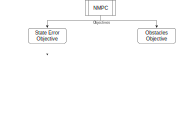
\includegraphics[scale=0.8]{pictures/mpc_planner_group/mpc_planner_1.pdf}}
		\centering
		\only<3>{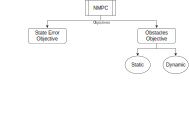
\includegraphics[scale=0.8]{pictures/mpc_planner_group/mpc_planner_2.pdf}}
		\centering
		\only<4>{\includegraphics[scale=0.8]{pictures/mpc_planner_group/mpc_planner_3.pdf}}
		\centering
		\only<5>{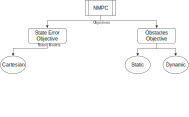
\includegraphics[scale=0.8]{pictures/mpc_planner_group/mpc_planner_4.pdf}}
		\centering
		\only<6>{\includegraphics[scale=0.8]{pictures/mpc_planner_group/mpc_planner_5.pdf}}
		\centering
		\only<7>{\includegraphics[scale=0.8]{pictures/mpc_planner_group/mpc_planner_6.pdf}}
	\end{frame}